% !TEX TS-program = pdflatex
% !TEX encoding = UTF-8 Unicode

% This is a simple template for a LaTeX document using the "article" class.
% See "book", "report", "letter" for other types of document.

\documentclass[12pt]{article} % use larger type; default would be 10pt

\usepackage[utf8]{inputenc} % set input encoding (not needed with XeLaTeX)

%%% Examples of Article customizations
% These packages are optional, depending whether you want the features they provide.
% See the LaTeX Companion or other references for full information.

%%% PAGE DIMENSIONS
\usepackage{geometry} % to change the page dimensions
\geometry{a4paper} % or letterpaper (US) or a5paper or....
% \geometry{margin=2in} % for example, change the margins to 2 inches all round
% \geometry{landscape} % set up the page for landscape
%   read geometry.pdf for detailed page layout information

\usepackage{graphicx} % support the \includegraphics command and options

% \usepackage[parfill]{parskip} % Activate to begin paragraphs with an empty line rather than an indent

%%% PACKAGES
\usepackage{booktabs} % for much better looking tables
\usepackage{array} % for better arrays (eg matrices) in maths
\usepackage{paralist} % very flexible & customisable lists (eg. enumerate/itemize, etc.)
\usepackage{verbatim} % adds environment for commenting out blocks of text & for better verbatim
\usepackage{subfig} % make it possible to include more than one captioned figure/table in a single float
% These packages are all incorporated in the memoir class to one degree or another...

%%% HEADERS & FOOTERS
\usepackage{fancyhdr} % This should be set AFTER setting up the page geometry
\pagestyle{fancy} % options: empty , plain , fancy
\renewcommand{\headrulewidth}{0pt} % customise the layout...
\lhead{}\chead{}\rhead{}
\lfoot{}\cfoot{\thepage}\rfoot{}

%%% SECTION TITLE APPEARANCE
\usepackage{sectsty}
\allsectionsfont{\sffamily\mdseries\upshape} % (See the fntguide.pdf for font help)
% (This matches ConTeXt defaults)

%%% ToC (table of contents) APPEARANCE
\usepackage[nottoc,notlof,notlot]{tocbibind} % Put the bibliography in the ToC
\usepackage[titles,subfigure]{tocloft} % Alter the style of the Table of Contents
\renewcommand{\cftsecfont}{\rmfamily\mdseries\upshape}
\renewcommand{\cftsecpagefont}{\rmfamily\mdseries\upshape} % No bold!

%%% END Article customizations

%%% The "real" document content comes below...

\title{Effects of the Injection of random variations of diverse artificial neurons during learning}

%\date{} % Activate to display a given date or no date (if empty),
         % otherwise the current date is printed 

\begin{document}
\maketitle

\section{Motivation}
To see the effects of injecting random artificial neural neurons generated with random transfer functions with varying parameters on the performance of artificial neural networks. 

The injections were made of random artificial neural networks just for convenience sake, but the goal was also to see if transfer functions complexification was indeed useful. Though this is not an act of complexification, rather it was increasing the variations of the artificial neural networks during optimization. In other words, what was being tested was the effects of increasing the variations of transfer functions in the population of neurons for co-evolution of artificial neural networks architectures with diverse transfer functions.

Related works include, COVNET, and SANE. However, both use fixed topologies for their neural network architecture. In this case, we are using a neural network with topology that can be mutated. This is done using flip-bit mutation. (* Draw diagram of the mutation process of the topology)
\section{Implementation}
The artificial neuron representation used for was \emph{self contained}. The activation function,$g(.)$, and the output function $f(.)$ together with the parameters of the output function (i.e $<p_1, p_2, p_3> $) were encoded together onto a genetic a single string. Thus, each neuron is  represented as  $n = <g(.),f(.), bias, p_1,p_2,p_3> $. The advantage of this is that it makes ensures that all the learned information by the neuron is self contained. As such cross-over operations, the randomness of cross-over is reduced. Also, it also keeps the genetic string shorter, which increases the likelihood of a more \emph{"meaning-full"} information cross-over. A \emph{meaning-full} cross-over is one that transmits the most amount of learned information to the other parent. In others words, if the ideal cross-over point on the genetic string is at $2$, then due to the shorter length of the genetic string (i.e. it not being concatenated with the whole genetic string representing the model), it is likely that the ideal cross-over that ensures the most cross-over of learned information is made. However, this is based on the assumption that a meaning-full cross-over is more effective.

Each node position $i$ in the neural network model has a population of candidate neurons $N_i =\{n_1,n_2...n_{max-pop} \}$. Other components such as the topology and weights between and in the layers also have a population of candidate topologies, and weights. In other words, There is a population of candidates for the inter-layer topology between input to hidden units $C_{ih}$, an intra-layer population of candidate of topologies for the hidden to hidden units $C_{hh}$, and finally, another population of candidates for the inter-layer topology  hidden to output units $C_{ho}$. Likewise, there are population of candidate weight matrices between these layers $W_{ih}, W_{hh}, W_{ho}$.
\section{Experimental setup}


The experiment was setup as follows:
\subsection{First Condition: Injection (Random)}
The first condition was to inject a set of randomly generated artificial neuron into the population of candidates for each node position. The transfer functions are random combinations of an activation function and an output function from the pool of transfer functions. The function parameters as well as the bias of the neurons are also randomly generated within their respective range. 

The injection of this set of random variations of nodes was done every generation during the optimization process, and was introduced (injected) into the population of candidate neurons. The population consisted of neurons which were offsprings of the old generations of neurons, post mutation and cross-over and some of neurons from older generations which have passed the selection process. In other words, the selection process selected from both the offsprings, and the parents.
\subsection{Second Condition: No Injection}
In the second condition, there was no injection of randomly generated sets of artificial neural network for any of the populations of the node positions. It solely relied the normal evolutionary operations, i.e. mutation and cross-over to create the variation of neurons. 
 \subsection{Benchmarks}
The datasets, with the exception of the Iris, where from the PROBEN1 Benchmark, which are standardized and make comparison of algorithms a lot more easier.
\section{Results and Discussions}
In general:
\begin{itemize}
\item In terms of performance, injecting random variations of artificial neurons into the populations of candidate neurons for the node positions improved performance significantly. This could be as a result of the increased exploratory behavior introduce as a result of the injection of random variations. This makes it more likely for the model to find the most appropriate variation of artificial neuron that best cooperates with the other components to form the suitable decision boundary. 

\item In terms of convergence, the results were also similar. Injection of random variations significantly improved the average convergence on the dataset. This is also likely due to the exploratory behavior of introducing random variations of artificial neurons. It is possible that the appropriate transfer function (i.e combination of activation and output function) is in the population of candidates, but not with the right configuration parameters (i.e. $<p_1,p_2,p_3>$). Thus, it doesn't become the appropriate variant needed. Also, it is possible that the the right combination of activation function and output function to produce the right transfer function is not in the population of candidates, as such; it will also make it an inappropriate variant. The introduction of a set of randomly generated artificial neurons increases the likelihood of the appropriate variant of artificial neuron being found. Thus, It is likely that the injection of random variations of artificial neurons could be helping learning by providing a mechanism for escaping local minima. Specifically, because the choice of the activation function and output function of the artificial doesn't undergo evolutionary operations, it is likely that the learning algorithm will be biased towards a certain region of the search space -as a result. However, introducing neurons with random combination of activation and output functions is likely to make it less biased, and more exploratory in its search for the appropriate model.

\item It is unlikely that the correct transfer function is not present, during initialisation phase, pre-optimisation, each population consists of all possible combination of the activation and output functions. 

\item The training and test error seem to be quite close, which suggests good generalization.

\end{itemize}


\begin{figure}[here]
 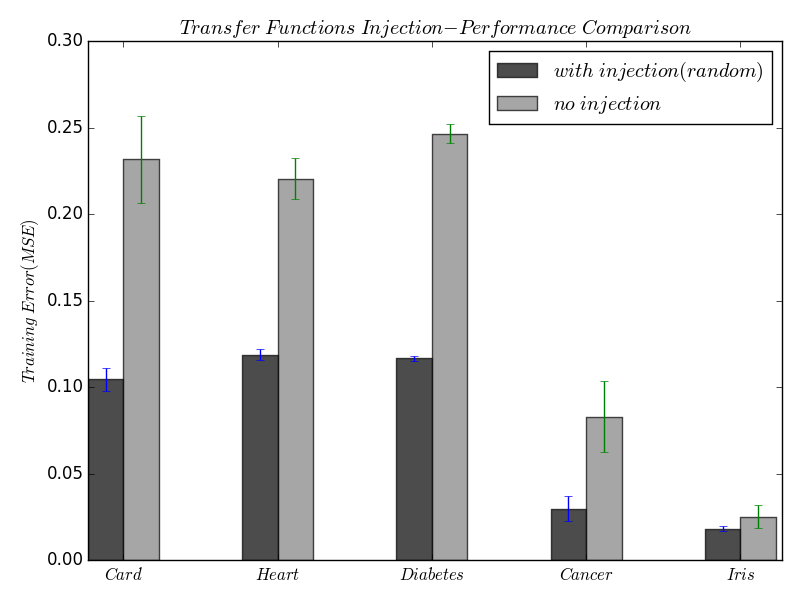
\includegraphics[scale=0.6]{errs_comp_inject_train.png}
 \caption{\label{comparison_injection} Results of the comparison in performance (MSE) in terms of training error between the two conditions: with injections of random variations of artificial neurons(in blue), and with no injection(in red).}
\end{figure}

\begin{figure}[here]
 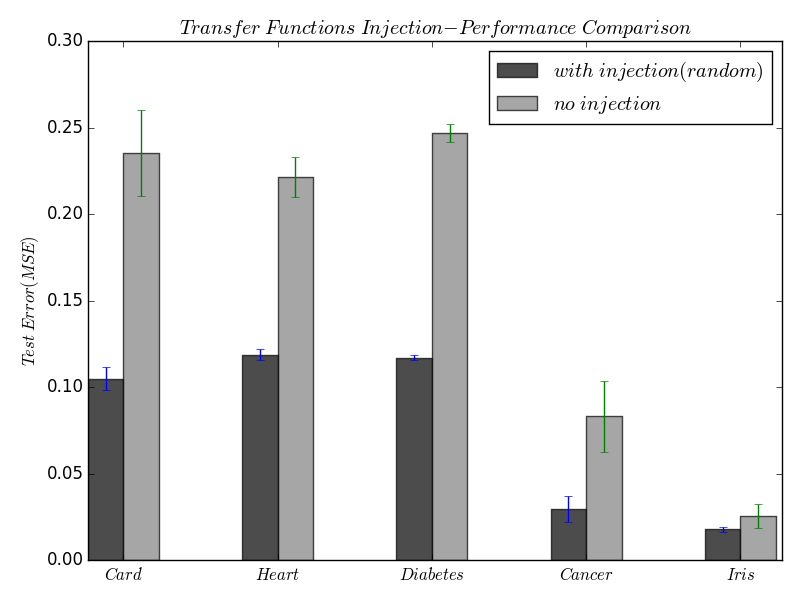
\includegraphics[scale=0.6]{errs_comp_inject_test.png}
 \caption{\label{comparison_injection} Results of the comparison in performance (MSE) in terms of training error between the two conditions: with injections of random variations of artificial neurons(in blue), and with no injection(in red).}
\end{figure}

\begin{figure}[here]
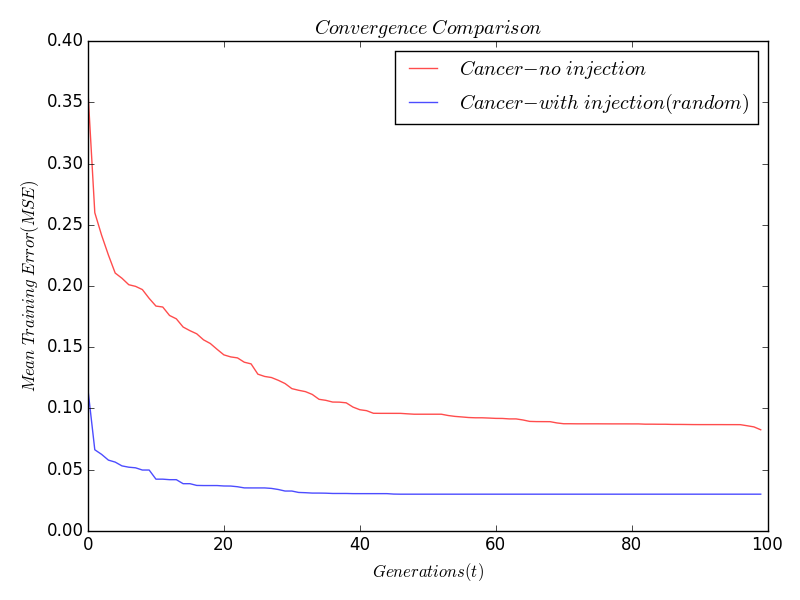
\includegraphics[scale=0.6]{errs_no_inject_convergence_Cancer.png}
\caption{\label{Convergence_cancer_injection} Comparison of convergence between the two conditions on the Breast Cancer dataset.}
\end{figure}


\begin{figure}[here]
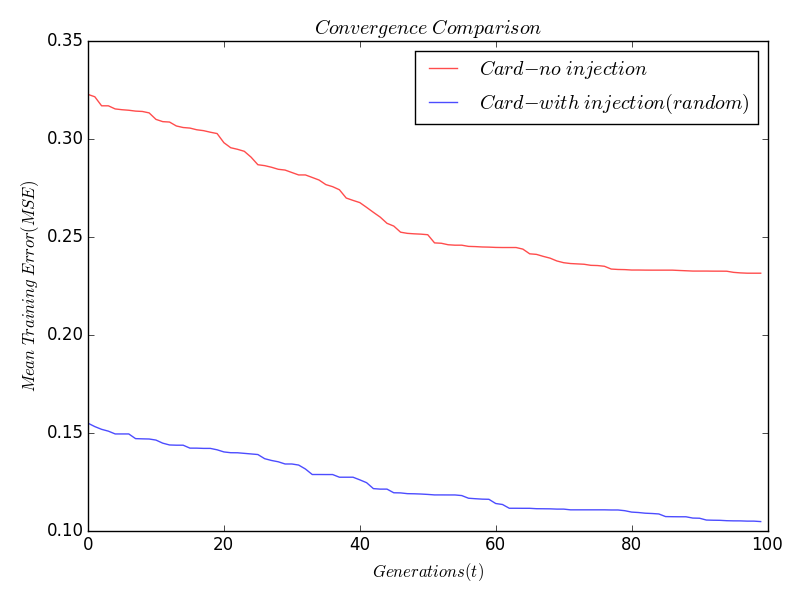
\includegraphics[scale=0.6]{errs_no_inject_convergence_Card.png}
\caption{\label{Convergence_cancer_injection} Comparison of convergence between the two conditions  on the Australian Credit Card dataset.}
\end{figure}

\begin{figure}[here]
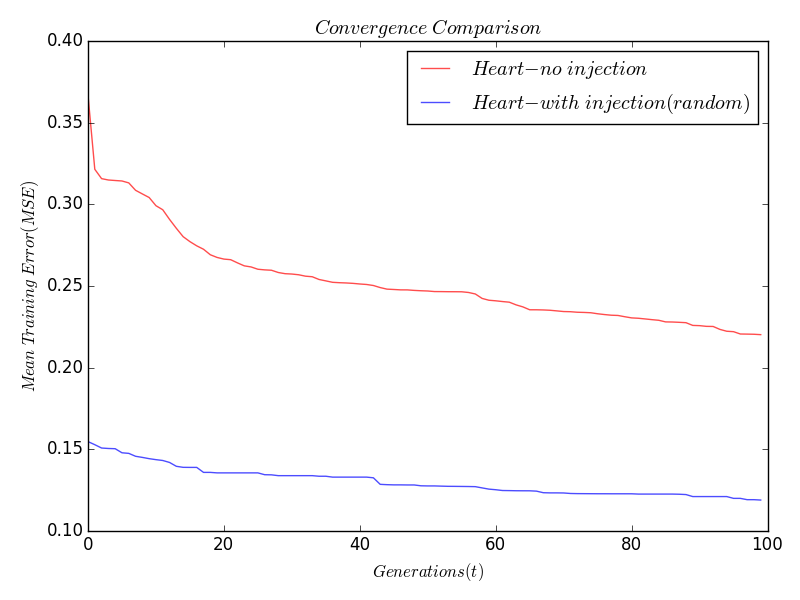
\includegraphics[scale=0.6]{errs_no_inject_convergence_Heart.png}
\caption{\label{Convergence_cancer_injection} Comparison of convergence between the two conditions on the Heart dataset. }
\end{figure}

\begin{figure}[here]
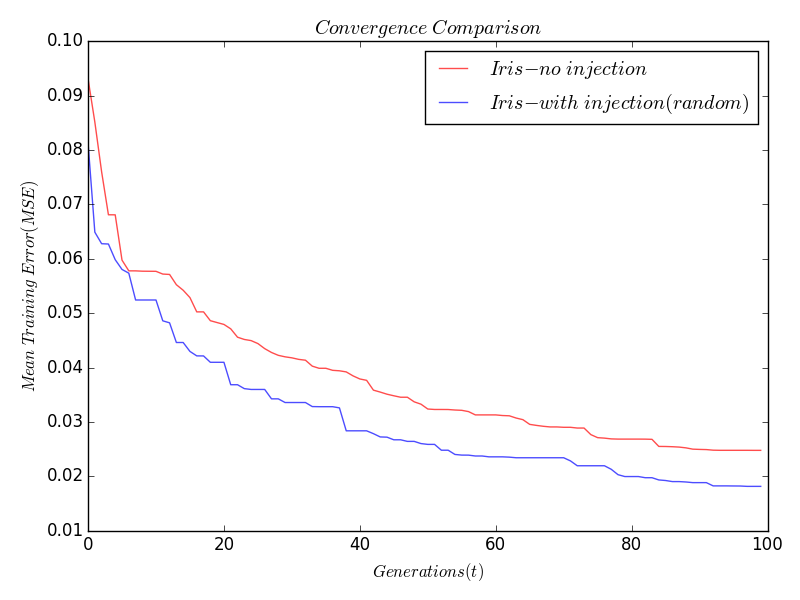
\includegraphics[scale=0.6]{errs_no_inject_convergence_Iris.png}
\caption{\label{Convergence_cancer_injection} Comparison of convergence between the two conditions on the Iris dataset.}
\end{figure}


\begin{figure}[here]
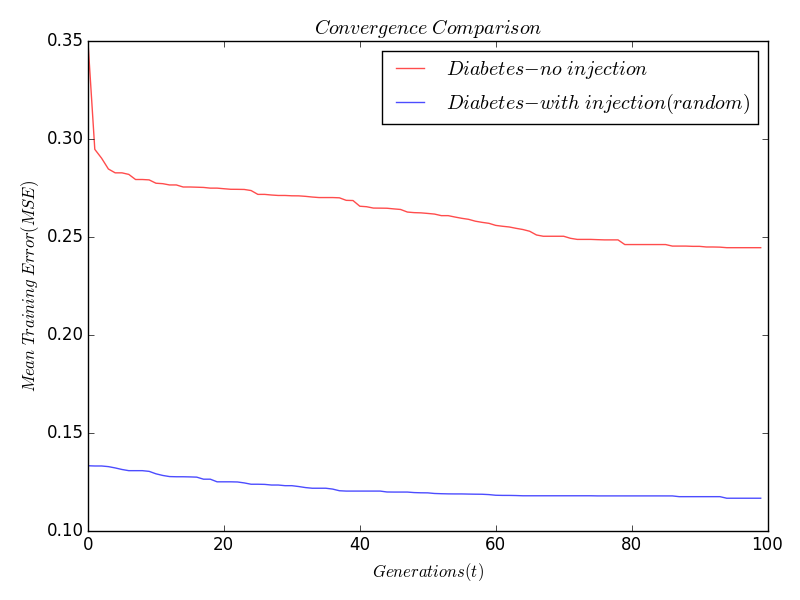
\includegraphics[scale=0.6]{errs_no_inject_convergence_Diabetes.png}
\caption{\label{Convergence_cancer_injection} Comparison of convergence between the two conditions on the Diabetes dataset.}
\end{figure}

\section{Conclusions}
In conclusion, the injection of random variations of transfer functions is improves both the convergence and generalization performance of co-evolutionary artificial neural network with diverse transfer functions. This is likely as a result of the exploratory behavior introduced by this mechanism, which helps to escape local minima.


\end{document}
